\documentclass[11pt]{book}
\usepackage{ifxetex}
\ifxetex
 \usepackage{fontspec}
  \usepackage{addfont}
 \usepackage{polyglossia}
 \setmainlanguage{italian}
 \usepackage[protrusion=true]{microtype}
\addfont{OT1}{tap}{tapir}
 \defaultfontfeatures{Ligatures=TeX}
  %\setmainfont{Josefin sans}
  \setmainfont{Minion Pro}
\else
 \usepackage[utf8]{inputenc}
 \usepackage[T1]{fontenc}
 \usepackage[italian]{babel}
 %\usepackage[osf]{libertine}
 \usepackage[light]{CormorantGaramond}
 \linespread{.9}
\fi
\usepackage[paperwidth=130mm,paperheight=210mm,top=12mm,bottom=25mm,outer=20mm,inner=13mm]{geometry}
\usepackage[]{matrita}
\usepackage{indentfirst}
\usepackage{graphicx}
\usepackage{pict2e}
\usepackage[object=vectorian]{pgfornament}%http://altermundus.com/pages/tkz/ornament/index.html
\usepackage{lettrine}
\usepackage{fancyhdr}
\usepackage{afterpage}
\usepackage{wasysym}
\pagestyle{fancy}
\pagenumbering{arabic}
\fancyhead{} % clear all header fields
\fancyfoot{} % clear all footer fields
\renewcommand{\headrulewidth}{0pt}
\renewcommand{\footrulewidth}{0pt}

\definecolor{commentcolor}{gray}{0.5}
\definecolor{etgray}{gray}{0.8}
\setlength{\afterpoemtitleskip}{2ex plus 0ex minus 1ex}
\setlength{\beforepoemtitleskip}{2.5ex plus 1ex minus 2ex}
\setlength{\leftmargini}{3em}
\setlength{\titleindent}{3em}
\renewcommand{\poemtitlefont}{\normalfont\large\bfseries}
\definecolor{crosscolor}{gray}{0.7}


\begin{document}
\newgeometry{left=15mm,right=15mm,top=20mm, bottom=30mm}
{%
\makeatletter
\let\strippt\strip@pt
\makeatother
\newcommand{\firstpageornament}{% 
\unitlength=1mm 

\begin{picture}(0,0)% 
\put(-19,13){\pgfornament[width=2cm]{37}}% 
\put(87,13){%
\pgfornament[width=2cm,symmetry=v]{37}}% 
\put(-19,-175){%
\pgfornament[width=2cm,symmetry=h]{37}}% 
\put(87,-175){% 
\pgfornament[width=2cm,symmetry=c]{37}}%
\end{picture}}% 

%\firstpageornament
}

\begin{center}
%\vspace*{\stretch{0.1}}
%\pgfornament[scale=.39]{72}\ {\Huge\textsf{matrita}}\ \pgfornament[scale=.39]{73}\\% 
%\pgfornament[scale=.6]{85}\\[5em]
%
%il pacchetto per creare il libretto delle nozze di\\[5em]

%{\Huge\hskip60pt\lower50pt\hbox{\itshape\usefont{OT1}{ppl}{m}{it}\textcolor{etgray}{\resizebox{35mm}{!}{\&}}} \hskip-175pt\sposa{} \hskip-20pt\lower40pt\hbox{\sposo}}

\begin{figure}
\vspace*{5cm}
\centering
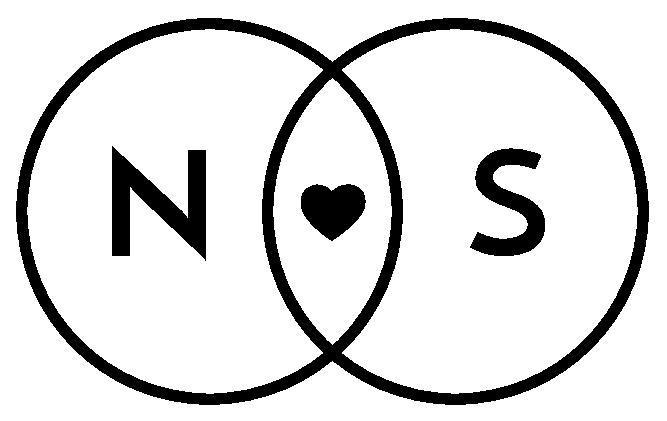
\includegraphics[scale=0.3]{img/Logo_piccolo.eps}

\huge \NSposo \ e \NSposa\\
\large 15 Settembre 2018\\
\end{figure}
\normalsize

\vspace*{\stretch{3}}
Parrochia di San Bernardo in Costalunga - Brescia

\end{center}
\restoregeometry
\clearpage
\afterpage{\cfoot{\thepage}}
%\end{document}
\null\vfill

%\begin{flushleft}
\begin{center}
{\footnotesize Questo libretto é stato creato con Amore e con \LaTeX}
\end{center}
%\end{flushleft}
\clearpage
\settowidth{\versewidth}{Il giorno al giorno ne affida il messaggio,}
\canztitle{I cieli narrano}
\begin{canzone}%[\versewidth]
\begin{ritornello}
I cieli narrano la gloria di Dio\\
e il firmamento annunzia l’opera sua,\\
Alleluja, alleluja, alleluja, allelu—u—ja!
\end{ritornello}

Il giorno al giorno ne affida il messaggio,\\
la notte alla notte ne trasmette notizia;\\
non è linguaggio, non sono parole\\
di cui non si oda il suono.

Là pose una tenda per il sole che sorge,\\
è come uno sposo dalla stanza nuziale,\\
esulta come un prode che corre\\
con gioia la sua strada.
\end{canzone}
%\vspace{-0.5\baselineskip}

\momento{Memoria del Battesimo}
\introduzione

\membatt

\vspace{-0.5\baselineskip}
\settowidth{\versewidth}{ti rendiamo grazie per la tua immensa gloria.}
\canztitle{Gloria}
\begin{canzone}%[versewidth]
\begin{ritornello}
Gloria a Dio nell'alto dei cieli\\
e pace in terra agli uomini che egli ama.
\end{ritornello}

Noi ti lodiamo, ti benediciamo,\\
ti adoriamo, ti glorifichiamo,\\
ti rendiamo grazie per la tua immensa gloria.\\
Signore Dio, re del cielo,\\
Dio Padre onnipotente.\\
Figlio unigenito, Cristo Gesù.

Signore Dio, Agnello di Dio,\\
Figlio del Padre, onnipotente\\
Tu che togli i peccati del mondo,\\
abbi pietà di noi,\\
Tu che togli i peccati del mondo,\\
accogli benigno la nostra preghiera,\\
Tu che siedi alla destra del Padre,\\
abbi pietà di noi.

Tu solo il Santo, tu solo il Signore,\\
Tu l'altissimo, Gesù Cristo.\\
Con lo Spirito Santo nella gloria del Padre.
\end{canzone}

\pagebreak
\momento{liturgia della parola}
\begin{lettura}{Dal Cantico dei Cantici}{Ct\,2,\,8--10.14.16a; 8,\,6--7a}
\lettrine[lines=3]{U}{na} voce! Il mio diletto!\\
Eccolo, viene\\
saltando per i monti,\\
balzando per le colline.\\
Somiglia il mio diletto a un capriolo\\
o ad un cerbiatto.\\
Eccolo, egli sta\\
dietro il nostro muro;\\
guarda dalla finestra,\\
spia attraverso le inferriate.\\

\noindent
Ora parla il mio diletto e mi dice:\\
«Alzati, amica mia,\\
mia bella, e vieni!\\
O mia colomba, che stai nelle fenditure della roccia,\\
nei nascondigli dei dirupi,\\
mostrami il tuo viso,\\
fammi sentire la tua voce,\\
perché la tua voce è soave,\\
il tuo viso è leggiadro».\\

\noindent
Il mio diletto è per me e io per lui.\\
Egli mi dice:\\
«Mettimi come sigillo sul tuo cuore,\\
come sigillo sul tuo braccio;\\
perché forte come la morte è l'amore,\\
tenace come gli inferi è la passione:\\
le sue vampe sono vampe di fuoco,\\
una fiamma del Signore!\\
Le grandi acque non possono spegnere l'amore\\
né i fiumi travolgerlo».\\
\end{lettura}

\pagebreak
\vspace{\baselineskip}
\renewcommand{\versettosalmo}{Il nostro Dio è grande nell'amore.}
\noindent\nomelibrofont{Salmo responsoriale {\small(Salmo 102)}}

\noindent\rispostasalmo

\nobreak
\begin{verse}
Benedici il Signore, anima mia,\\
quanto è in me benedica il suo santo nome.\\
Benedici il Signore, anima mia,\\
non dimenticare tanti suoi benefici.\\
\rispostasalmo

Buono e pietoso è il Signore,\\
lento all'ira e grande nell'amore.\\
Come un padre ha pietà dei suoi figli,\\
così il Signore ha pietà di quanti lo temono.\\
\rispostasalmo

La grazia del Signore è da sempre,\\
dura in eterno per quanti lo temono;\\
la sua giustizia per i figli dei figli,\\
per quanti custodiscono la sua alleanza.\\
\rispostasalmo
\end{verse}

\begin{lettura}{Dalla prima lettera di san Paolo apostolo ai Corinzi\\}{Co\,12, 31-13, 8a}
\lettrine[lines=3]{F}{ratelli}, aspirate ai carismi più grandi! E io vi mostrerò una via migliore di tutte.\\

Se anche parlassi le lingue degli uomini e degli angeli, ma non avessi la carità, sono come un bronzo che risuona o un cembalo che tintinna.\\

E se avessi il dono della profezia e conoscessi tutti i misteri e tutta la scienza, e possedessi la pienezza della fede così da trasportare le montagne, ma non avessi la carità, non sono nulla.\\

E se anche distribuissi tutte le mie sostanze e dessi il mio corpo per esser bruciato, ma non avessi la carità, niente mi giova.\\

La carità è paziente, è benigna la carità; non è invidiosa la carità, non si vanta, non si gonfia, non manca di rispetto, non cerca il suo interesse, non si adira, non tiene conto del male ricevuto, non gode dell'ingiustizia, ma si compiace della verità. Tutto copre, tutto crede, tutto spera, tutto sopporta.\\

La carità non avrà mai fine.\\
\end{lettura}

\canztitle{Alleluia Irlandese (di Lécot)}
\settowidth{\versewidth}{Alleluia alleluia alleluia alleluia}
\begin{canzone}%[versewidth]
\begin{ritornello}
Alleluia, alleluia,\\
alleluia; alleluia\\
\end{ritornello}

Cantate al Signore con gioia,\\
grandi prodigi ha compiuto!
\end{canzone}
\begin{vangelo}{Matteo}{Mt\,7, 21.24-29}
\lettrine[lines=3]{I}{\,n} quel tempo, Gesù disse ai suoi discepoli:\\
<<Non chiunque mi dice: "Signore, Signore", entrerà nel regno dei cieli, ma colui che fa la volontà del Padre mio che è nei cieli.\\

Perciò chiunque ascolta queste mie parole e le mette  in pratica, è simile a un uomo saggio che ha costruito la sua casa sulla roccia. Cadde la pioggia, strariparono i fiumi, soffiarono i venti e si abbatterono su quella casa, ed essa non cadde, perché era fondata sopra la roccia.\\

Chiunque ascolta queste mie parole e non le mette in pratica, è simile a un uomo stolto che ha costruito la sua casa sulla sabbia.\\
Cadde la pioggia, strariparono i fiumi, soffiarono i venti e si abbatterono su quella casa, ed essa cadde, e la sua rovina fu grande>>\\

Quando Gesù ebbe finito questi discorsi, le folle restarono stupite del suo insegnamento: egli infatti insegnava loro come uno che ha autorità e non come i loro scribi.
\end{vangelo}

\momento{Rito del Matrimonio}
\matrintro
\medskip

\matrpre
\medskip

\consintro
\medskip

\promesse
\medskip

\preghpost


\momento{Scambio degli anelli}
\benedizioneanelli

\medskip

\consegnanello
%\vfill
%\settowidth{\versewidth}{Per la luna e per le stelle,}
%\canztitle{Canzone da definire 2}
%\begin{canzone}%[versewidth]
%\begin{ritornello}
%Lorem ipsum,\\
%Lorem ipsum,\\
%Lorem ipsum,\\
%Lorem ipsum
%\end{ritornello}
%
%Lorem ipsum,\\
%Lorem ipsum,\\
%Lorem ipsum,\\
%Lorem ipsum.
%
%Lorem ipsum,\\
%Lorem ipsum,\\
%Lorem ipsum,\\
%Lorem ipsum.
%\end{canzone}
\linebreak
\begin{center}

\includegraphics[scale=0.1]{img/cuori_venn.eps}
\end{center}
\vfill
\pagebreak
\momento{Preghiere dei fedeli}
\introfedeli
\preghierefedeli
\vfill
\pagebreak

% No litanie
%\introlitanie
%\litanie

\momento{Liturgia Eucaristica}
Accogli, Signore, i doni e le preghiere che Ti presentiamo
per \sposa{} e \sposo, uniti nel vincolo
santo: questo mistero, che esprime la pienezza della
tua carità, custodisca per sempre il loro amore. \par\nobreak
Per Cristo nostro Signore.
\rispostatutti{Amen}

\settowidth{\versewidth}{Et Benedictus Fructus Ventris,}
\canztitle{Ave Maria (Bach - Gounod)}
\begin{canzone}%[versewidth]
Ave Maria, Gratia plena,\\
Maria Gratia Plena\\
Maria Gratia Plena\\
Ave, ave Dominus\\
Dominus Tecum.\\
Benedicta Tu In Mulieribus\\
Et Benedictos,\\
Et Benedictus Fructus Ventris,\\
Ventris tui, Jesus\\
Ave Maria!\\
\end{canzone}

\settowidth{\versewidth}{Osanna, osanna, osanna nell'alto dei cieli.}
\canztitle{Santo (Bonfitto)}
\begin{canzone}%[versewidth]
Santo,\\
Santo,\\
Santo il Signore\\
Dio dell'universo.

I cieli e la terra\\
sono pieni della tua gloria.

\begin{ritornello}
Osanna, Osanna, Osanna nell'alto dei cieli.
\end{ritornello}

Benedetto\\
colui che viene\\
nel nome del Signore.

\begin{ritornello}
Osanna, Osanna, Osanna nell'alto dei cieli.
\end{ritornello}

\end{canzone}

%\momento{Benedizione degli sposi}
%\benedizionesposi[1]

%\momento{Rito della Pace}

%\newpage
\vfill
\pagebreak
\momento{Comunione}
\settowidth{\versewidth}{ma che son parte di una immensa vita,}
\canztitle{Dolce sentire}
\begin{canzone}%[versewidth]
Dolce sentire come nel mio cuore\\
ora umilmente, sta nascendo amore.\\
Dolce è capire che non son più solo,\\
ma che son parte di una immensa vita,\\
che generosa risplende intorno a me:\\
dono di Lui, del suo immenso amor.

Ci ha dato il cielo e le chiare stelle,\\
fratello sole e sorella luna,\\
la madre terra con frutti, prati e fiori,\\
il fuoco, il vento, l'aria e l'acqua pura,\\
fonte di vita, per le sue creature:\\
dono di Lui, del suo immenso amor,\\
dono di Lui, del suo immenso amor.

Sia laudato nostro Signore,\\
che ha creato l'universo intero.\\
Sia laudato nostro Signore,\\
noi tutti siamo sue creature:\\
dono di Lui, del suo immenso amor.\\
Beato chi lo serve in umiltà.
\end{canzone}

\momento{Benedizione finale}
\benedizionefinale

\congedo

\momento{Canti Finali}
\settowidth{\versewidth}{Ain't no valley low, ain't no river wide enough baby}
\canztitle{Hallelujah di Leonard Cohen}
\begin{canzone}%[versewidth]
Now, I've heard there was a secret chord\\
That David played, and it pleased the Lord\\
But you don't really care for music, do you?\\
It goes like this, the fourth, the fifth\\
The minor fall, the major lift\\
The baffled king composing hallelujah

\begin{ritornello}
Hallelujah, hallelujah, hallelujah, hallelujah 
\end{ritornello}

Your faith was strong but you needed proof\\
You saw her bathing on the roof\\
Her beauty and the moonlight overthrew ya\\
She tied you to a kitchen chair\\
She broke your throne, and she cut your hair\\
And from your lips she drew the hallelujah

\begin{ritornello}
Hallelujah, hallelujah, hallelujah, hallelujah
\end{ritornello}

You say I took the name in vain\\
I don't even know the name\\
But if I did, well really, what's it to you?\\
There's a blaze of light in every word\\
It doesn't matter which you heard\\
The holy or the broken hallelujah

\begin{ritornello}
Hallelujah, hallelujah, hallelujah, hallelujah
\end{ritornello}

I did my best, it wasn't much\\
I couldn't feel, so I tried to touch\\
I've told the truth, I didn't come to fool you\\
And even though it all went wrong\\
I'll stand before the lord of song\\
With nothing on my tongue but hallelujah

\begin{ritornello}
Hallelujah, hallelujah, hallelujah, hallelujah\dots
\end{ritornello}
\end{canzone}

\settowidth{\versewidth}{Ain't no valley low, ain't no river wide enough baby}
\canztitle{Ain't No Mountain High Enough}
\begin{canzone}%[versewidth]
Listen baby, ain't no mountain high\\
Ain't no valley low,\\
Ain't no river wide enough baby\\
If you need me call me no matter where you are\\
No matter how far don't worry baby\\
Just call my name I'll be there in a hurry\\
You don't have to worry

\begin{ritornello}
'Cause baby there ain't no mountain high enough\\
Ain't no valley low enough\\
Ain't no river wide enough\\
To keep me from getting to you babe
\end{ritornello}

Remember the day I set you free\\
I told you you could always count on me darling\\
From that day on, I made a vow\\
I'll be there when you want me\\
Some way, some how

\begin{ritornello}
'Cause baby there ain't no mountain high enough\\
Ain't no valley low enough\\
Ain't no river wide enough\\
To keep me from getting to you babe
\end{ritornello}

Oh no darling\\
No wind, no rain\\
Or winters cold can stop me baby, na na baby\\
'Cause you are my goal\\
If you're ever in trouble\\
I'll be there on the double\\
Just send for me, oh baby, ha

My love is alive\\
Way down in my heart\\
Although we are miles apart\\
If you ever need a helping hand\\
I'll be there on the double\\
Just as fast as I can\\
Don't you know that there

\begin{ritornello}
Ain't no mountain high enough\\
Ain't no valley low enough\\
Ain't no river wide enough\\
To keep me from getting to you babe
\end{ritornello}

Don'tcha know that there\\
Ain't no mountain high enough\\
Ain't no valley low enough\\
Ain't no river wide enough\\
Ain't mountain high enough\\
Ain't no valley low enough
\end{canzone}
\vfill
\begin{center}

\includegraphics[scale=0.1]{img/cuori_venn.eps}\\
%{\footnotesize Questo libretto é stato creato con Amore e con \LaTeX.}
\end{center}
\begin{quotation}\small\selectlanguage{italian}
Sono tre le parole che si devono dire sempre, tre parole che devono essere nella casa: \emph{permesso, grazie, scusa.}\\Le tre parole magiche. Con queste tre parole, con la preghiera dello sposo per la sposa e viceversa, con fare la pace sempre prima che finisca la giornata, il matrimonio andrà avanti.
\begin{flushright}Papa Francesco, 2 aprile 2014\end{flushright}
\end{quotation}

\end{document}
